\documentclass[11pt,xcolor={dvipsnames},hyperref={pdftex,pdfpagemode=UseNone,hidelinks,pdfdisplaydoctitle=true},usepdftitle=false]{beamer}
\usepackage{presentation}

\usepackage{tikz}
\usepackage{tikz-cd}

\usetikzlibrary{arrows,
	arrows.meta,
  backgrounds,
	bending,
	calc,
	decorations,
  decorations.markings,
	decorations.pathmorphing,
  fit,
  hobby,
	matrix,
	shapes}

\definecolor{harvestgold}{rgb}{0.85, 0.57, 0.0}
\definecolor{pakistangreen}{rgb}{0.0, 0.4, 0.0}
\definecolor{rosewood}{rgb}{0.4, 0.0, 0.04}
\definecolor{sangria}{rgb}{0.57, 0.0, 0.04}
\definecolor{taupe}{rgb}{0.28, 0.24, 0.2}
\definecolor{tealgreen}{rgb}{0.0, 0.51, 0.5}
\definecolor{ultramarine}{rgb}{0.07, 0.04, 0.56}

\renewcommand{\AA}{\mathbf{A}}
\newcommand{\BB}{\mathbf{B}}
\newcommand{\CC}{\mathbf{C}}
\newcommand{\DD}{\mathbf{D}}
\newcommand{\EE}{\mathbf{E}}
\newcommand{\FF}{\mathbf{F}}
\newcommand{\GG}{\mathbf{G}}
\newcommand{\RR}{\mathbf{R}}
\newcommand{\XX}{\mathbf{X}}

\newcommand{\angs}[1]{\langle #1 \rangle}
\newcommand{\enquine}[1]{\ulcorner {#1} \urcorner}

\newcommand{\leftboxtensor}{\mathbin{\underline{\boxtimes}}}
\newcommand{\leftsemidirect}{\mathbin{\underline{\rtimes}}}
\newcommand{\leftsum}{\mathbin{\underline{\oplus}}}
\newcommand{\lefttensor}{\mathbin{\underline{\otimes}}}
\newcommand{\rightboxtensor}{\mathbin{\overline{\boxtimes}}}
\newcommand{\rightsemidirect}{\mathbin{\overline{\rtimes}}}
\newcommand{\rightsum}{\mathbin{\overline{\oplus}}}
\newcommand{\righttensor}{\mathbin{\overline{\otimes}}}

\newcommand{\coPi}{\rotatebox[origin=c]{180}{$\Pi$}}
\newcommand{\op}{\textit{op}}

% Enter presentation title to populate PDF metadata:
\hypersetup{pdftitle={Cographs, twofold symmetric monoidal structures, and factorization algebras}}

% Enter path to PDF file with figures:
\newcommand{\pdf}{figures.pdf}

\begin{document}

% Enter title:
\title{Cographs, twofold symmetric monoidal structures, \& factorization algebras}

\information
[https://clarkbar.github.io/papers/facts.pdf]
{Clark Barwick, The University of Edinburgh}
{CT2025, Brno -- 16 July 2025}

\frame{\titlepage}

\begin{frame}
  \frametitle{locality}
  \textsb{Locality}: measurements made in a region of spacetime should not depend upon measurements performed in a \textsb{distant} region of spacetime. (Haag, Haag--Kastler)

  \bigskip

  More refined: the cluster decomposition principle. (Weinberg)

  \bigskip

  \textsb{Factorization algebras} allow us to combine observables in spacetime regions that are sufficiently \textsb{apart}.
\end{frame}

\begin{frame}
  \frametitle{same \& different}
  \textsb{Homotopy theory} studies \textsb{sameness} as a \textsb{structure} rather than a \textsb{property}.

  \bigskip

  Let $X$ be a space and $x,y \in X$.
  The \textsb{path space} $\enquine{x \sim y}$ is the space of ways for $x$ and $y$ to be the same.
  These path spaces are then assembled in combinatorially useful ways.

  \bigskip

  Let's try to study \textsb{difference} or \textsb{apartness} in the same way.
  We'll call it \textsb{isolation theory}.
  We'll define spaces $\enquine{x \nsim y}$ of ways for $x$ and $y$ to be \textsb{different}.
  We'll assemble these spaces in combinatorially useful ways.
\end{frame}

\begin{frame}
  \frametitle{example}
  Consider a manifold $M$, and consider its homotopy type $\Pi(M)$.
  Let $x,y \in M$.
  The path space is the fiber of the diagonal
  \[
  \begin{tikzcd}[ampersand replacement=\&]
    \enquine{x \sim y} \arrow[d] \arrow[r] \& \Pi(\Delta_M) \arrow[d] \\
    \{(x,y)\} \arrow[r] \& \Pi(M \times M)
  \end{tikzcd}
  \]

  Note: if $M = \mathbf{R}^n$, then $\enquine{x \sim y}$ is always contractible, even if $x \neq y$.
\end{frame}

\begin{frame}
  \frametitle{example -- continued}
  Let us define this dual thing as the fiber of the \textsb{complement} of the diagonal:
  \[
  \begin{tikzcd}[ampersand replacement=\&]
    \enquine{x \nsim y} \arrow[d] \arrow[r] \& \Pi(M \times M - \Delta_M) \arrow[d] \\
    \{(x,y)\} \arrow[r] \& \Pi(M \times M)
  \end{tikzcd}
  \]

  Note: if $M = \mathbf{R}^n$, then $\enquine{x \nsim y}$ is always $S^{n-1}$, even if $x = y$.

  \bigskip

  Let's now think about how to assemble these spaces combinatorially.
\end{frame}

\begin{frame}
  \frametitle{graphs}
  \textsb{Graph} $(V,E)$: a pair consisting of
  \begin{itemize}
    \item a finite set $V$ of \textsb{vertices}
    \item a set $E \subseteq {V \choose 2}$ of \textsb{edges}
  \end{itemize}
  \textsb{Morphism} $(V,E) \to (V',E')$: a map $f \colon V \to V'$ such that
  \[
    \{a,b\} \in E \implies \{f(a),f(b)\} \in E'
  \]
\end{frame}

\begin{frame}
  \frametitle{notation}

  $\angs{n} =$ the graph with $n$ vertices and no edges
  \begin{center}
  \begin{tikzpicture}
    \tikzstyle{vertex}=[circle,fill=black,minimum size=4pt,inner sep=0pt]
    \node[vertex] (v_1) at (1,0) {};
    \node[vertex] (v_2) at (0.309,0.951) {};
    \node[vertex] (v_3) at (-0.809,0.588)  {};
    \node[vertex] (v_4) at (-0.809,-0.588)  {};
    \node[vertex] (v_5) at (0.309,-0.951)  {};
  \end{tikzpicture}
  \end{center}
  
  We disallow loops!
  So there is no morphism from $K_2 = 
    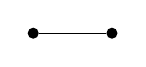
\begin{tikzpicture}
      \tikzstyle{vertex}=[circle,fill=black,minimum size=4pt,inner sep=0pt]
      \node[vertex] (v_1) at (0,0) {};
      \node[vertex] (v_2) at (1,0)  {};
      \draw (v_1) -- (v_2);
      \node[fit=(current bounding box),inner sep=0mm]{};
    \end{tikzpicture}
    $ to $\angs{1}$.
\end{frame}

\begin{frame}
  \frametitle{sums}
  If $A$ and $B$ are two graphs, we can add them in two ways:
  \begin{itemize}
    \item disconnected sum, or coproduct: $A \leftsum B$
    \item connected sum, or join: $A \rightsum B$
  \end{itemize}

  \begin{example}
    \[
      \angs{2 \leftsum 3}=\ 
      \begin{tikzpicture}[baseline=0]
        \tikzstyle{vertex}=[circle,fill=black,minimum size=4pt,inner sep=0pt]
        \node[vertex] (v_1) at (-0.5,-0.5) {};
        \node[vertex] (v_2) at (-0.5,0.5) {};
        \node[vertex] (v_3) at (0.5,-1)  {};
        \node[vertex] (v_4) at (0.5,0)  {};
        \node[vertex] (v_5) at (0.5,1)  {};
      \end{tikzpicture}
      = \angs{5}
      \qquad
      \angs{2 \rightsum 3}=\ 
      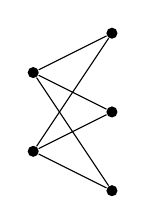
\begin{tikzpicture}[baseline=0]
        \tikzstyle{vertex}=[circle,fill=black,minimum size=4pt,inner sep=0pt]
        \node[vertex] (v_1) at (-0.5,-0.5) {};
        \node[vertex] (v_2) at (-0.5,0.5) {};
        \node[vertex] (v_3) at (0.5,-1)  {};
        \node[vertex] (v_4) at (0.5,0)  {};
        \node[vertex] (v_5) at (0.5,1)  {};
        \draw (v_1) -- (v_3) -- (v_2) -- (v_4) -- (v_1) -- cycle;
        \draw (v_1) -- (v_5) -- (v_2) -- cycle;
      \end{tikzpicture}
      = K_{2,3}
    \]
  \end{example}
\end{frame}

\begin{frame}
  \frametitle{fun}
  \[
    \angs{1 \rightsum (1 \leftsum (1 \rightsum (1 \leftsum (1 \rightsum 1))))} =
    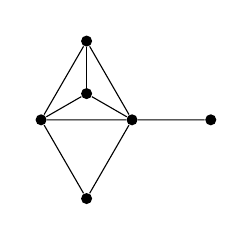
\begin{tikzpicture}[baseline=0]
      \tikzstyle{vertex}=[circle,fill=black,minimum size=4pt,inner sep=0pt]
      \node[vertex] (v_1) at (-1.155,0) {};
      \node[vertex] (v_2) at (-0.577,1) {};
      \node[vertex] (v_3) at (-0.577,0.333) {};
      \node[vertex] (v_4) at (-0.577,-1) {};
      \node[vertex] (v_5) at (0,0) {};
      \node[vertex] (v_6) at (1,0) {};
      \draw (v_5) -- (v_2) -- (v_1) -- (v_3) -- (v_5) -- (v_1) -- (v_4) -- (v_5) -- (v_6) -- cycle;
      \draw (v_2) -- (v_3) -- cycle;
      \node[fit=(current bounding box),inner sep=1mm]{};
    \end{tikzpicture}
  \]
\end{frame}

\begin{frame}
  \frametitle{twofold symmetric monoidal structures}
  The sums $\leftsum, \rightsum$ are symmetric monoidal structures with the same unit, $\angs{0} = \varnothing$.

  There is also a natural intertwiner
  \[
    (A \rightsum B) \leftsum (C \rightsum D) \to (A \leftsum C) \rightsum (B \leftsum D)
  \]
  which exhibits
  \begin{itemize}
    \item $\rightsum$ as lax symmetric monoidal with respect to $\leftsum$ and
    \item $\leftsum$ as colax symmetric monoidal with respect to $\rightsum$.
  \end{itemize}

  In other words, the category of graphs is a \textsb{twofold symmetric monoidal category}.
\end{frame}

\begin{frame}
  \frametitle{cographs}
  A \textsb{cograph} is a graph in which the following implication holds for all vertices $a,b,c,d$:
  \[
    \{\{a,b\}, \{b,c\}, \{c,d\}\} \subseteq E \implies \{\{a,c\}, \{a,d\}, \{b,d\}\} \cap E \neq \varnothing
  \]
  \[
    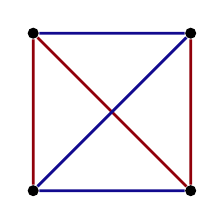
\begin{tikzpicture}[baseline=0]
      \tikzstyle{vertex}=[circle,fill=black,minimum size=4pt,inner sep=0pt]
      \node[vertex] (v_1) at (-1,-1) {};
      \node[vertex] (v_2) at (-1,1) {};
      \node[vertex] (v_3) at (1,-1)  {};
      \node[vertex] (v_4) at (1,1)  {};
      \draw[color=sangria,line width = 1pt] (v_1) -- (v_2) -- (v_3) -- (v_4);
      \draw[color=ultramarine,line width = 1pt] (v_3) -- (v_1) -- (v_4) -- (v_2); 
    \end{tikzpicture}
  \]

  \textsb{Fun fact}: cographs $=$ graphs that can be presented using
  \[
    \angs{1},
    \quad
    \leftsum,
    \quad
    \rightsum
  \]

  \bigskip

  (\textsb{co} is an unfortunate shortening of \textsb{complement reducible}.)
\end{frame}

\begin{frame}
  \frametitle{universal property}
  $\DD =$ the twofold symmetric monoidal category of cographs 

  $\angs{1} \in \mathrm{CMon}(\DD,\leftsum)$

  \begin{theorem}
    $\DD$ is the free twofold symmetric monoidal category on a commutative monoid for the left tensor product:
    \[
      \mathrm{TwofoldSMF}((\DD,\leftsum,\rightsum),(\CC,\lefttensor,\righttensor)) = \mathrm{CMon}(\CC,\lefttensor) 
    \]
  \end{theorem}
\end{frame}

\begin{frame}
  \frametitle{example}
  Let's return to our manifold $M$.

  For every cograph $\angs{\lambda}$, consider the space
  \[
    M^{\lambda} = \{ x \in M^{V\angs{\lambda}} : \{a,b\} \in E\angs{\lambda} \implies x_a \neq x_b\}
  \]
  The assignment $\angs{\lambda} \mapsto M^{\lambda}$ is a functor $\DD^{\op} \to \textbf{Man}$.

  \[
    M^n = M \times \cdots \times M
  \]
  
  \[
    M^{1 \rightsum 1} = M \times M - \Delta_M
  \]
\end{frame}

\begin{frame}
  \frametitle{isolability structures}
  Consider an inclusion $\angs{\lambda} \subseteq \angs{\lambda'}$ of a full (`induced') subgraph,
  and let $\angs{\lambda} \to \angs{\mu}$ be any morphism that is surjective on vertices.
  Then there's a pushout
  \[
    \begin{tikzcd}[ampersand replacement=\&]
      \angs{\lambda} \arrow[->>,d] \arrow[right hook->,r] \& \angs{\lambda'} \arrow[->>,d] \\
      \angs{\mu} \arrow[right hook->,r] \& \angs{\mu'}
    \end{tikzcd}
  \]
  in $\DD$.

  An \textsb{isolability object} of a category $\XX$ is a functor $\DD^{\op} \to \XX$ such that all pushout squares as above in $\DD$ are carried to pullback squares in $\XX$.
\end{frame}

\begin{frame}
  \frametitle{isolability objects}
  An \textsb{isolability object} of a category $\XX$ is a functor $\DD^{\op} \to \XX$ such that all pushout squares as above in $\DD$ are carried to pullback squares in $\XX$.

  The assignment $\angs{\lambda} \to M^{\lambda}$ is an isolability manifold.

  Passing to (stratified) homotopy types gives us an isolability (stratified) \textsb{anima}.


\end{frame}

\begin{frame}
  \frametitle{Sheaves on isolability spaces}
\end{frame}

\begin{frame}
  \frametitle{Factorization algebras in quite a lot of generality}
\end{frame}

\end{document}
